\documentclass[a4paper, 11pt]{article}

\usepackage{graphicx}
\usepackage[francais]{babel}
\usepackage[utf8]{inputenc}
\usepackage[T1]{fontenc}
\usepackage{listings}

\lstset{language={Python},}


\begin{document}

\title{Rapport du projet de RO}
\author{Paul Bonaud\\
  Victor Godayer}
\date\today

\maketitle

\begin{abstract}
  Ce projet implante une solution de décryptage face à un chiffre
  polyalphabétique périodique .

  Ce décryptage se réalise selon plusieurs étapes que nous décrirons
  dans le présent rapport.
\end{abstract}
\newpage
\tableofcontents
\newpage


\section{Introduction}
Notre travail se compartimente en 3 parties, selon le sujet fourni.

\paragraph{}
Dans un premier temps nous avons aborder le problème de la période.
Trouver la période revient à trouver le nombre d'alphabets utilisés pour
coder le texte clair.

\paragraph{}
Dans un second temps, il nous est nécessaire de rechercher des cribles
dans le chiffre, ceci nous permettant d'établir un lien entre les
lettres du crible et les alphabets.

La qualité de la recherche du crible s'appuie essentiellement sur
trois \textit{indicateurs} : la \textit{pertinence}, la
\textit{rareté} et la \textit{vraissemblance}.

\paragraph{}
Enfin il nous était demandé d'avoir une approche de programmation génétique pour
pouvoir retrouver complètement les alphabets servant à chiffrer le
texte clair. Cependant nous n'avons pas eu le temps de nous consacrer
pleinement à cette tâche. Nous presenterons donc seulement nos
reflexions sur le sujet.


\section{Conception}

\subsection{Choix du langage}
Nous connaissions le langage \textit{Python}.
Ce dernier étant partiulièrement bien adapté pour la manipulation
du type de donnée \textit{string}, nous l'avons choisi pour implanter
le projet.
Appartenant à la catégorie des langages fonctionnels, c'est également
un aspect pratique pour le projet.

\subsection{Détermination de la période}

\subsubsection{Méthode courte}
Nous avons implanté la méthode de Kasiski courte de la manière
suivante.

Pour un texte chiffré et une taille \textit{l} donnée la fonction recherche toutes
les sous-chaines de la taille \textit{l} qui se répetent dans le texte
chiffré.

Une fonction de test se charge de tester toutes les valeurs de l
intéressantes.
Pour voir les résultats des tests se reporter à la partie test.

\paragraph{}
Voici le code python (très accessible) de cette fonction:
\newpage
\begin{lstlisting}
def kasiski_court(text, l):
    for i in range(len(text)-l):
        target = text[i:i+l]
        found = text[i+l:].find(target)
        if found != -1:
            f = found+i+l
            if i>0 and text[i-1:i+l] == text[f-1:f+l]:
                continue
            if i+l < len(text) and text[i:i+l+1] == text[f:f+l+1]:
                continue            

            print '\%-10s \%3d' \% (target, found+l)
\end{lstlisting}


\subsubsection{Méthode longue}
La methode longue a été implanter en suivant le cours n 11 de LANAKI.

Voici en quelques mots ce que réalise notre programme:
\begin{itemize}
\item Récupère toutes les distances-lettres possibles du chiffre.
\item Pour tout facteur entre 1 et 48 :
  \begin{itemize}
  \item compter le nombre de fois dont ce facteur est un diviseur des
    distances.
  \end{itemize}
\item Enfin pondérer chaque sous-totaux obtenus par leur facteur
  respectif.
\end{itemize}

La période est alors le facteur pour lequel le total est maximum. Ou
tout du moins quasiment maximum.\\
Pour laisser un peu de liberte a l'utilisateur, nous avons pris les
maximums obtenus et lui avons laisser le choix de la période à
choisir.\\

Des tests et exemples d'éxécution de ce programme sont disponibles
dans la section tests.


\subsection{Recherche de crible}

Comme nous n'avons pas pu mener à bout cette partie, la problématique
de la présentation du résultat n'a même pas eu être aborder.
Voici les \textit{recherches} et codages que nous avons effectué sur
les notions de pertinence et de rareté.

\subsubsection{Pertinence}
Même après avoir réfléchis longuement sur cette notion nous n'avons
pas pu établir un indicateur réellement fiable pour un crible donné.
Nous n'avons pas réussi à trouver des règles claires nous permettant
d'évaluer la pertinence du crible en fonction d'une période.

Comme un exemple vaut mieux qu'un long discours, se reporter à la
partie test pour voir les résultats de la fonction pertinence.


\subsubsection{Rareté}
Pour la rareté du crible nous avons, pour une table de
fréquence donnée, calculé une valeur entre 0 et 1, 0 représentant une
rareté nulle et 1 une rareté maximale.

La rareté du crible se fait simplement en sommant les fréquences
d'apparition de chaque lettre puis en divisant cette somme par le
nombre de lettre multiplié par la fréquence maximale pour la table des
fréquences donnée.

C'est une sorte de moyenne des fréquences des lettres qui constituent
le mot.

\subsubsection{Vraissemblance}
Nous n'avons pas réussi à établir une fonction d'évaluation de la
vraisemblance d'une position d'un crible.

Cependant nous avons codé une fonction \textit{table\_frequences} qui, à un
crible et une période données, nous renvoie une liste de la longueur
de la \textit{période}.

On nommera cette liste \textit{l}.

Chaque élément de \texit{l}, est une liste des
lettres qui se trouvent à une position \textit{j} dans le crible, modulo
la valeur de la \textit{période}.

Nous appelerons cette seconde liste \textit{l$'$}

Chaque \textit{l'} listent des couples contenant la lettre et son
occurrence. L'occurrence est en le nombre de fois ou on a trouvé cette
lettre à la position \textit{j} modulo la \textit{période}

Voir dans la partie test pour avoir des exemples clairs.



\subsection{Reconstitution du chiffre}

\begin{itemize}
\item Quelle est votre définition du volume mémoriel ?
\item Quelle est votre définition de l'ADN ?
\item Comment se déroulent les croisements ?
\item Qu'avez vous testé ?
\end{itemize}


\subsubsection{Volume mémoriel}

Pour valuer le volume mémoriel d'UN alphabet nous avons eu comme idée
de regarder les espaces deux-à-deux entre les lettres de
l'alphabet. Puis de compter le nombre d'espacement différents dans
cette alphabet.\\
Ainsi plus les lettres sont espacés de manières aléatoires, plus
l'alphabet est dur à retenir et par conséquent son volume memoriel
augmente.
\textit{Nous avons implanter cette fonction de volume mémoriel pour UN
alphabet. Les exemples d'éxécution sont disponibles dans la section
tests.\\}

Il faut ensuite réfléchir à l'idée de volume mémoriel pour un ensemble
d'alphabet.\\
Par exemple si l'alphabet est répété plusieurs fois et seulement
décalé, le volume mémoriel pour l'ensemble des alphabets n'est pas
énorme. Il suffit de connaitre les décalages des alphabets (par
exemple : avec un mot clef comme dans l'exemple du sujet). L'idée ici
est donc de comparer les alphabets (aux décalages près): plus ils sont "éloignés", plus le
volume mémoriel augmente.



\subsubsection{Programmation génétique}
En pensant utile de vous montrer ceci le jour des tests, nous avons
implanté la methode proposée par M. Marthon pour casser des vigenères
simples (Avec clé). Avec le calcul d'Indice de Coincidence Mutelle. \\

Le programme realisé est \textbf{casser\_chiffre\_vigenere}.

Des tests de ce programme se trouvent dans la section test.\\


Ce qui suit sont nos réfléxions sur les algorithmes génétiques que nous aurions
pu implanter.\\
\begin{itemize}
\item \textbf{ADN et croisements}

Nous pensions garder les lettres et leur ordre pour définir l'ADN d'un alphabet.

Nous avons commencé a implanter deux fonctions pour modifier les ADNs: \textit{mutation} et \textit{croisement}.
Celles-ci sont disponibles dans le fichier \textbf{genetique.py}.

Voici l'explication de ces deux fontions:

\underline{mutation(alphabet, niveau)}
Cette fonction fait muter certaines parties d'un alphabet. Une
mutation étant un échange de deux lettres dans l'alphabet. Le paramètre
\textit{niveau} détermine le nombre de mutations à effectuer.

\underline{croisement(alphabet1, alphabet2)}
Nous avons penser a faire un croisement entre deux alphabets, on
choisissant aléatoirement une moitié de l'un des deux. Puis d'échanger
les lettres une à une avec cette moitié. Voici un schéma qui
expliquera mieux qu'un discours avec deux alphabets Alphabet1 et
Alphabet2. Le résultat est le fils à la fin du schéma.
 
\begin{center}
 \scalebox{0.6}[0.6]{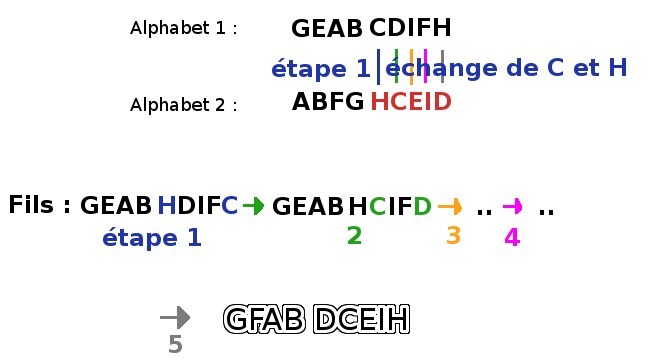
\includegraphics{./croisement.jpg}}
\end{center}


\item \textbf{Séléction artificielle}
On peut sélectionner les individus en fonction du volume mémoriel de
chacun. Sachant qu'on cherche a minimiser ce volume mémoriel et
essayer de retrouver les alphabets.

\item \textbf{Conclusion}
Bien sûr la taille des populations, le nombre de croisements, de
mutations ne peut être évalué que par l'expérimentation. Encore une
fois c'est dommage de ne pas avoir pu finir l'implantation pour
tester. Mais on peut penser que avec une valuation totale du texte
clair, les algorithmes génétiques auraient pu trouver la solution de
la clé alphabétique. \\

Associer au travail sur les cribles, on pourrait sûrement
obtenir des résultats intéressants.

\end{itemize}



\section{Tests}

\subsection{Détermination de la période}

\subsubsection{Méthode courte}

Les longueurs possible des sous chaines sont automatiquement testées
dans le programme de test.
Celles-ci vont de la longueur du texte divisé par 2 à 2.

\begin{lstlisting}
\$ python kasiski_court.py
text? -> texte exemple de la jangada
...
...
test d'une longueur de sous chaine de:5
test d'une longueur de sous chaine de:4
DDQF       186 # distance entre les sous chaines repétées
KYUU        12
test d'une longueur de sous chaine de:3
RYM        192
TOZ        186
RPL         60
HHH         54

détermination de la période: pgcd de [186, 12, 192, 186, 60, 54] =
6
\end{lstlisting}

\subsubsection{Méthode longue}
...

Premiere exemple sur la jangada: (Periode attendu : 6)
\begin{lstlisting}
moore:~/Travail/2A/RO/cryptox> python kasiski_long.py 
phyjs  lyddq fdzxg asgzz qqehx gkfnd rxuju giocy tdxvk sbxhhuypoh  dvyry mhuhp uydkj oxphe tozsl etnpm vffov pdpaj xhyynojygg  aymeq ynfuq lnmvl yfgsu zmqiz tlbqg yugsq eubvn rcredgruzb  lrmxy uhqhp zdrrg crohe pqxuf ivvrp lphon thvdd qfhqsntzhh  hnfep mqkyu uexkt ogzgk yuumf vijdq dpzjq sykrp lxhxqrymvk  lohhh otozv dkspp suvjh d

Here are the period values possible:
[6, 12]

Which one do you wan't to choose? (0,1,..,1)
0

6
\end{lstlisting}

Deuxieme exemple provenant de Lanaki: (Periode attendu : 7)
\begin{lstlisting}
moore:~/Travail/2A/RO/cryptox> python kasiski_long.py 

RNQJH  AUKGV  WGIVO  BBSEJ  CRYUS  FMQLP  OFTLCMRHKB BUTNA  WXZQS  NFWLM  OHYOF  VMKTV  HKVPKKSWEI  TGSRB LNAGJ  BFLAM  EAEJW  WVGZG  SVLBKIXHGT  JKYUC  HLKTU MWWK

7
\end{lstlisting}


\subsection{Crible}

\subsubsection{Pertinence}
Ces tests ne tiennent pas forcément compte du fait que le crible est
un mot avec du sens.
Pour mettre à rude épreuve la logique de la fonction il était plus
simple d'employer une séquence de lettres avec des répétitions aux
endroits qui nous intéressait.

\begin{lstlisting}
>> p = 6 # la periode
>> pertinence('soldats',p)
>> 1.0
>> pertinence('soldatso',p)
>> 1.0 # Ici on pourrait s'attendre à un indicateur plus eleve
\end{lstlisting}

\subsubsection{Rareté}
Voici sous forme d'un tableau la rareté obtenu pour différent crible
de tests : \\

\begin{tabular}{|c|c|c|c|c|}
  \hline
   ``soldats'' & ``escorte'' & ``zebre'' & ``legerement'' & ``wagon'' \\
  \hline
   0.535415100974 & 0.406934585165 & 0.49089956356 & 0.38087729338 & 0.692843895006  \\
  \hline
\end{tabular}

\subsubsection{Vraisemblance}

Le premier paramètre de la fonction est le crible et le seconde la période

\begin{lstlisting}
>>> from crible import *
>>> table_frequences("soldats",6)
[('s', 2), ('o', 1), ('l', 1), ('d', 1), ('a', 1), ('t', 1)]

>>> table_frequences("onomatope",6)
[('o', 2), ('p', 1, 'n', 1), ('e', 1, 'o', 1), ('m', 1), ('a', 1),
  ('t', 1)]

>>> table_frequences("tagadaga",2)
[('t', 1, 'g', 2, 'd', 1), ('a', 4)]
\end{lstlisting}


\subsection{Reconstitution du chiffre}

\begin{lstlisting}
moore:~/Travail/2A/RO/cryptox> ./casser_chiffre_vigenere.py exemples/mystere_chiffre 

Chiffre : CE JGB FVNA WGG CA KZCFV DC ECAUE TS AVVUF HOEKAOéW ;
QNI CPSQHE PMFGR VN êBJS FZ BQWB CFUZNI, DLE KWIK DêMM IIV JOVL ZRJ PTMG
QZFNAQVCEA à UCAKEVLSE VN BGIGV ACLFR THWKS A’FNB HCVET KGIGLMM V’SA UéSQJSE GLCK EH’ZLA WB BET.
MF EHFI QD B’RJT XSG IIAQKSZSLITZR HUM LCHJ SM LFBDPMFH : ZRIA HZHKôT KWZN KéMWAUAV QCW ZN
GUQKGNECM VS OZEV BITVR ML RVJTQFUHVR TW JERI L’SJRT LM XOHO, QCA SFK PZGDEVMMFH PV QC’GB AFMUW
ZR SOV KSAJ OC DO ERIAGB, RJT VSHHIETDSZVNB éYOYV EV LCHJ LMK VBDMMK ; SG RIVKW DLE TS
RVMEZKWGé UE VGG BGIVACAJ NM NWRET XSG QV CM IIR CEA MBF JOVL DYLS ZSWFFNVSPYVS YMS YVS
IMHEVS, USWF JECDSZVNB VS PV QCW BBLS KGBQLIAGBF EOA HSAJéEA HOE UIDWFFVS DGWRJ, EB FS
PFNAARéEFNA HOF CEA EêARJ CPGGRJ. CIJ QR E’EAL DNJ AAKSM U’ADGWE C’EAHFVK BWF, ANZS TW
DEZNKADNC EAL RR C’AXHZVHUMJ PVVN. TWG CCUA YFNEDMK âARJ SWFH PRPITZRJ DMK DYLS OJOAUS DAQRJ
ACKGV SIMF EHV DMK DYLS OJOAUEA NSEKUA ; WH PVUF IIV EE USFPYEVL EHV FWJH YVNBWARET XWIIVNB
SJNECMJ PRRUKGIC UADSBGRGM, K’WYJ SCAJRET BGIWFUZK ZR URWAH PYEUAB, DLE VW TBET KWIK HUQ
UCHIEVL SG HUQ K’SA éCOQYBRET.

Here are the period values possible:
[6, 12]
Which one do you wan't to choose? (0,1,..,1)
0

Cle : RAISON
Text : LE BON SENS EST LA CHOSE DU MONDE LA MIEUX PARTAGéE ;
CAR CHACUN PENSE EN êTRE SI BIEN POURVU, QUE CEUX MêME QUI SONT LES PLUS
DIFFICILES à CONTENTER EN TOUTE AUTRE CHOSE N’ONT POINT COUTUME D’EN DéSIRER PLUS QU’ILS EN ONT.
EN QUOI IL N’EST PAS VRAISEMBLABLE QUE TOUS SE TROMPENT : MAIS PLUTôT CELA TéMOIGNE QUE LA
PUISSANCE DE BIEN JUGER ET DISTINGUER LE VRAI D’AVEC LE FAUX, QUI EST PROPREMENT CE QU’ON NOMME
LE BON SENS OU LA RAISON, EST NATURELLEMENT éGALE EN TOUS LES HOMMES ; ET AINSI QUE LA
DIVERSITé DE NOS OPINIONS NE VIENT PAS DE CE QUE LES UNS SONT PLUS RAISONNABLES QUE LES
AUTRES, MAIS SEULEMENT DE CE QUE NOUS CONDUISONS NOS PENSéES PAR DIVERSES VOIES, ET NE
CONSIDéRONS PAS LES MêMES CHOSES. CAR CE N’EST PAS ASSEZ D’AVOIR L’ESPRIT BON, MAIS LE
PRINCIPAL EST DE L’APPLIQUER BIEN. LES PLUS GRANDES âMES SONT CAPABLES DES PLUS GRANDS VICES
AUSSI BIEN QUE DES PLUS GRANDES VERTUS ; ET CEUX QUI NE MARCHENT QUE FORT LENTEMENT PEUVENT
AVANCER BEAUCOUP DAVANTAGE, S’ILS SUIVENT TOUJOURS LE DROIT CHEMIN, QUE NE FONT CEUX QUI
COURENT ET QUI S’EN éLOIGNENT.
\end{lstlisting}

\section{Conclusion}

Le sujet de ce projet nous a beacoup plus, bien qu'il soit long.
Meme si nous n'avons pas pu le mené à sa fin, il nous a permis de nous
plonger dans le domaine de la cryptologie.
En deça, les spécifications étant assez large, nous avons du prendre
un certains nombre de décision.
Cette liberté accordée était une motivation de plus pour dans la
réalisation de ce projet.



\end{document}
